\documentclass[graphics]{beamer}

\usepackage{graphicx}
\usepackage{verbatim}
\usepackage{wrapfig}
\useoutertheme{shadow}
%\usecolortheme{orchid}
\usecolortheme{seahorse}


% math commands
\newcommand{\be}{\begin{eqnarray}}
\newcommand{\ee}{\end{eqnarray}}
\newcommand{\beq}{\begin{equation}}
\newcommand{\eeq}{\end{equation}}
\def\simless{\mathbin{\lower 3pt\hbox
      {$\rlap{\raise 5pt\hbox{$\char'074$}}\mathchar"7218$}}}
\def\simgreat{\mathbin{\lower 3pt\hbox
      {$\rlap{\raise 5pt\hbox{$\char'076$}}\mathchar"7218$}}} %> or of order

% variables

\def\toonscale{0.45}
\def\mboxy#1{\mbox{\small #1}}


\begin{comment}
\AtBeginSection[]{
  \frame{
    \frametitle{Outline}
    \tableofcontents[currentsection]
  }
}
\end{comment}

\title{Coherent cosmology with FRBs
}
%\subtitle{interim update}
\author[U. Pen]{Ue-Li Pen and collaborators (D. Jow, O. Wucknitz, ++)
}
\date{Feb 10, 2023}


\begin{document}

%\section*{Introduction}
\section{Lenses}

\begin{comment}
  \subsection{Outline}

  \frame{
    \frametitle{Outline}
    \tableofcontents
  }
\end{comment}

\frame{\maketitle}


  \frame{
    \frametitle{Coherent radiation}
    \begin{itemize}
        \item Coherent, distant source of radiation
        \item Interference effects under multi-path propagation
        \item potential for diffraction limited measurements: planet masses
        \item sensitive to ns time delay propagating for gigaparsecs
        \item corresponds to strain $h \ll 10^{-26}$: far exceeds LIGO
        \item highly elongated antenna pattern: sensitive to
          longitudinal modes          
    \end{itemize}
  }


  \frame{
\vspace{-0.25in}
    \frametitle{FRB110523}
%\hspace{2.5in}
\includegraphics[width=2.5in]{Figures/scint110523.png}
\includegraphics[width=1.75in]{Figures/corr110523.png}
Masui++ 2015, Nature, 528, 523
  }


  \frame{
%\vspace{-0.25in}
    \frametitle{Scintillometry VLBI}
\hspace{-0.25in}
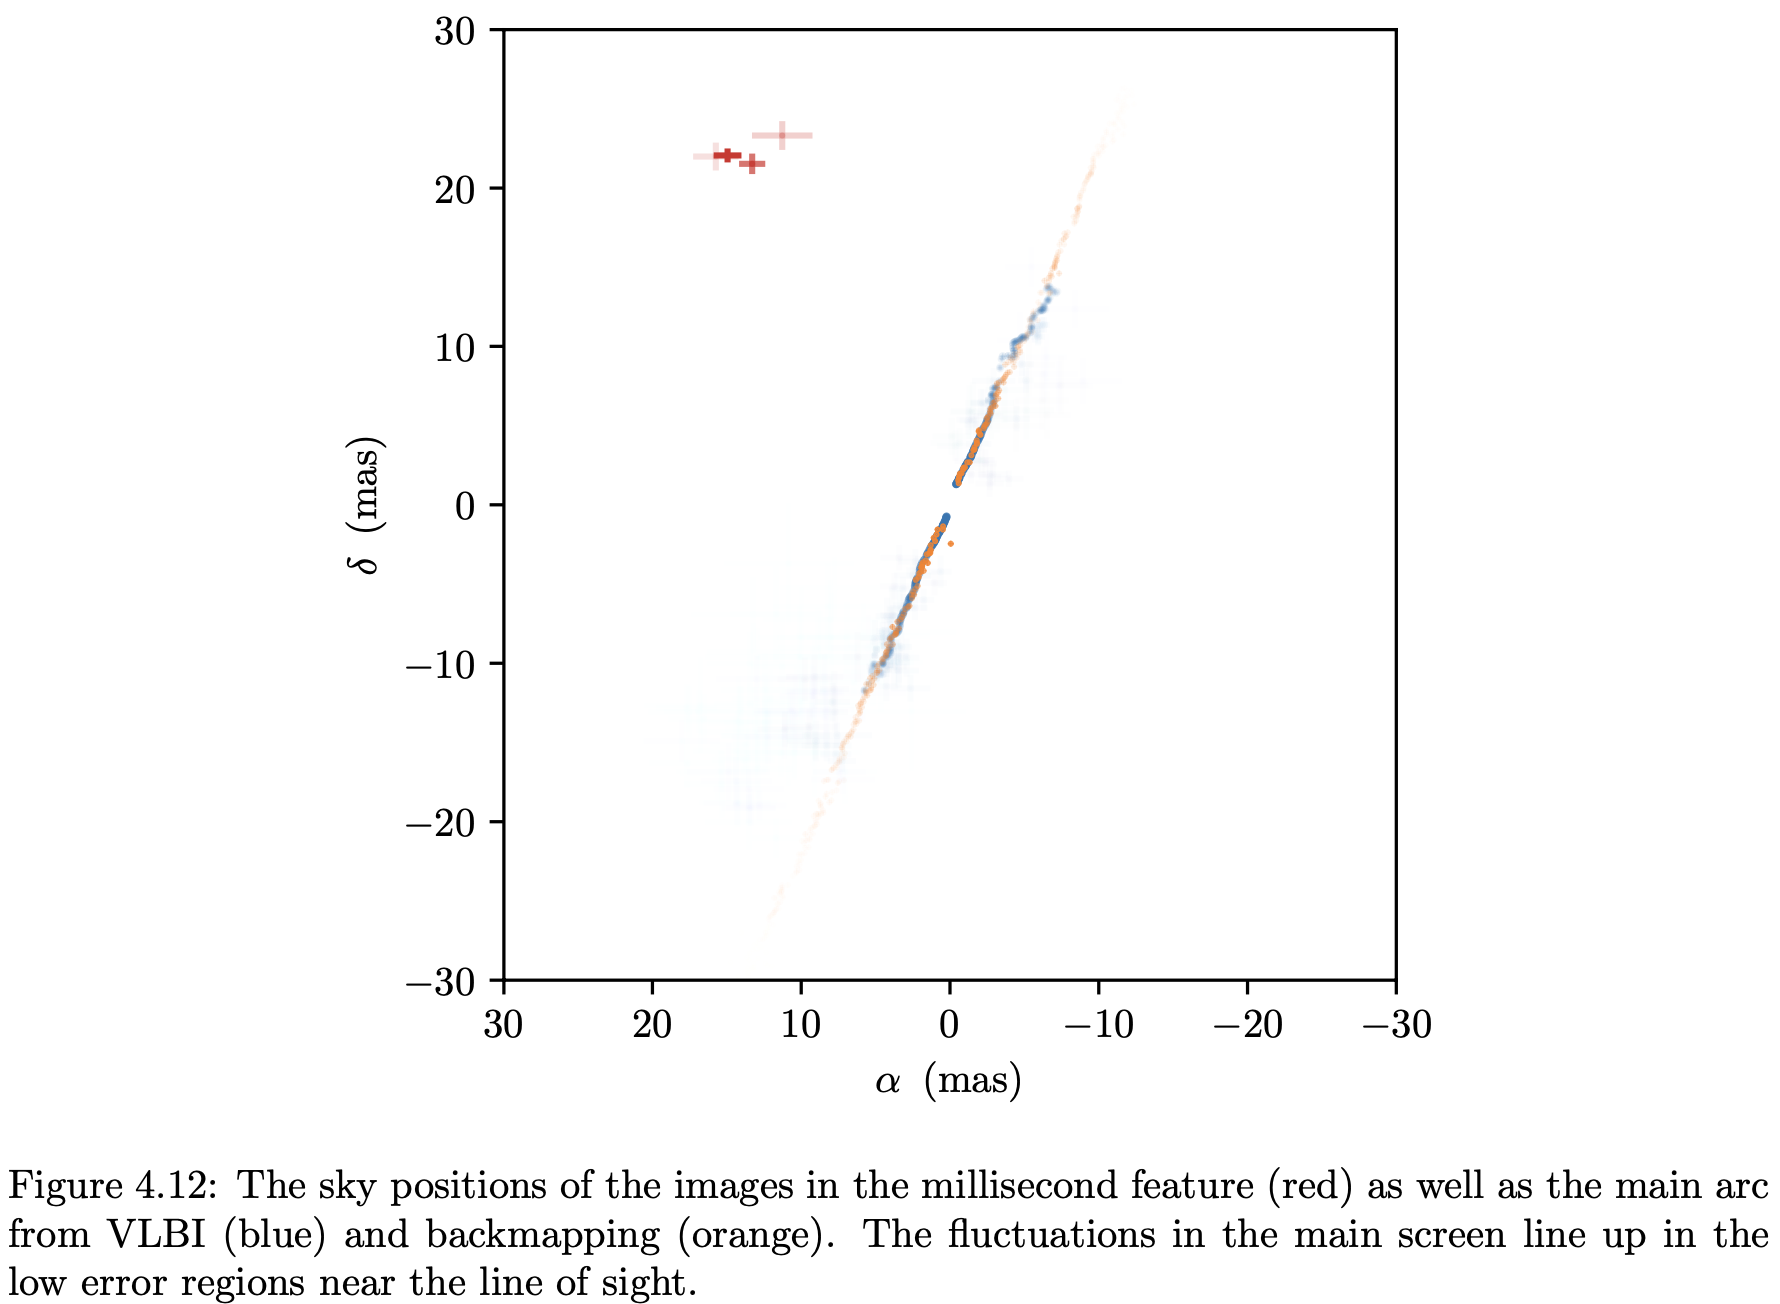
\includegraphics[width=3.5in]{Figures/VLBI0834.png}
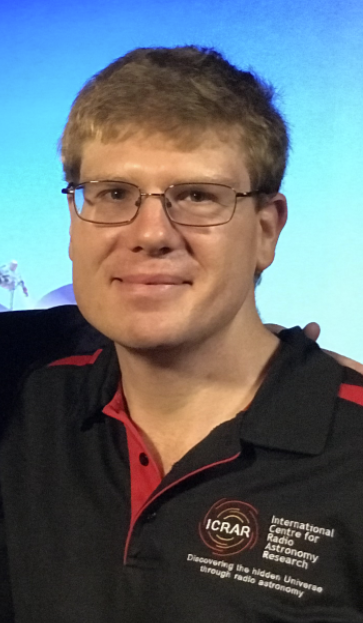
\includegraphics[width=1.05in]{Figures/jpm.png}

Baker++ .  In memoriam J-P Macquart.
  }


  

  \frame{

    \frametitle{ precision astrometry}
%\vspace{-0.25in}
\begin{center}
%\hspace{-0.5in}
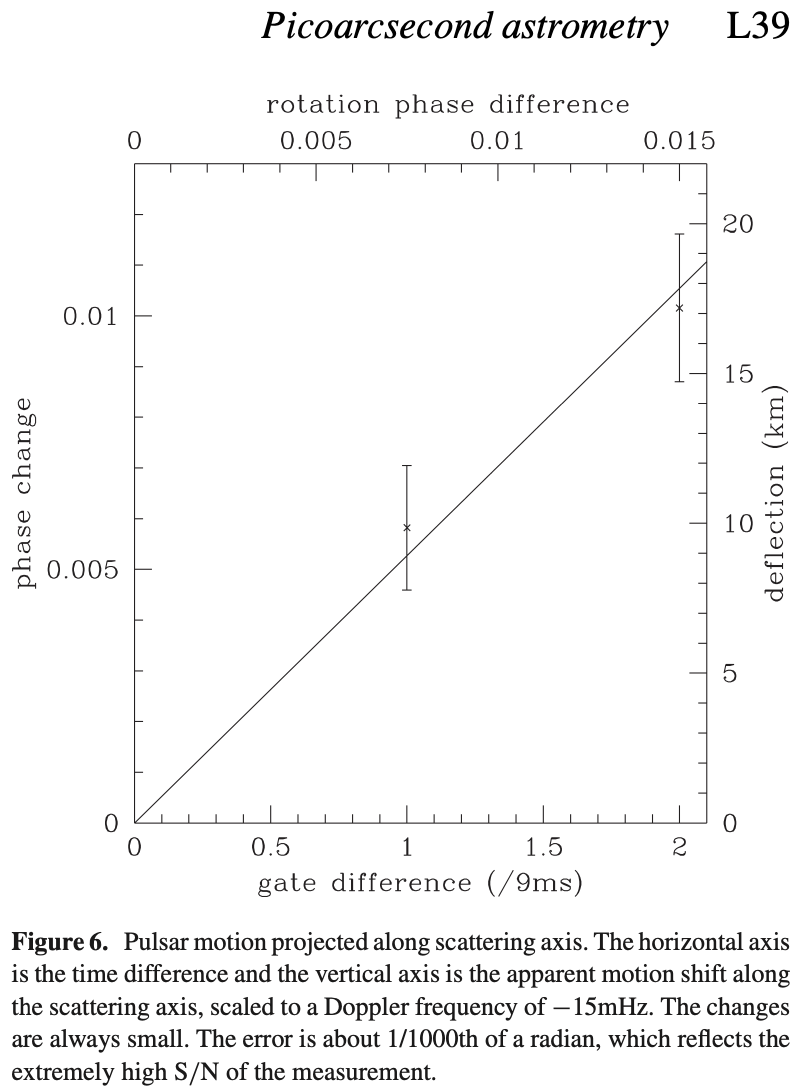
\includegraphics[width=2.05in]{Figures/pico.png}
UP+14
\end{center}
  }


  \frame{
\vspace{-0.5in}
    \frametitle{New Observables}
    \begin{itemize}
    \item for coherent sources: FRBs, pulsars
    \item weak lensing: imaginary image allows time delay measurement (Jow+21)
    \item strong lensing: delay measurements enable measurement of
      co-linearity (Jow++21)
    \item microlensing: instant time delay, planets (Jow+20)
    \item macrolensing: potentially nano-second delay -- universe
      expands!  Dark energy, etc (Wucknitz+21)
    \item dimensionless strain cm/Gigalightyears $h\sim \Delta t/t \sim 10^{-26}$:
      competitive with LIGO, etc
    \end{itemize}
  }


\frame{
  \frametitle{Time delay}
    \begin{itemize}
      \item electric field interference pattern
      \item time delay to nanoseconds
      \item flux ratio
      \item instant microlensing mass
   \end{itemize}
}

\frame{
  \frametitle{Macro, Plasma lensing}
    \begin{itemize}
     \item most FRBs are plasma lensed: scintillation/scattering observed
      \item use plasma lenses cosmologically
   \end{itemize}
}


  \frame{
%\vspace{-0.25in}
    \frametitle{Macro lensing}
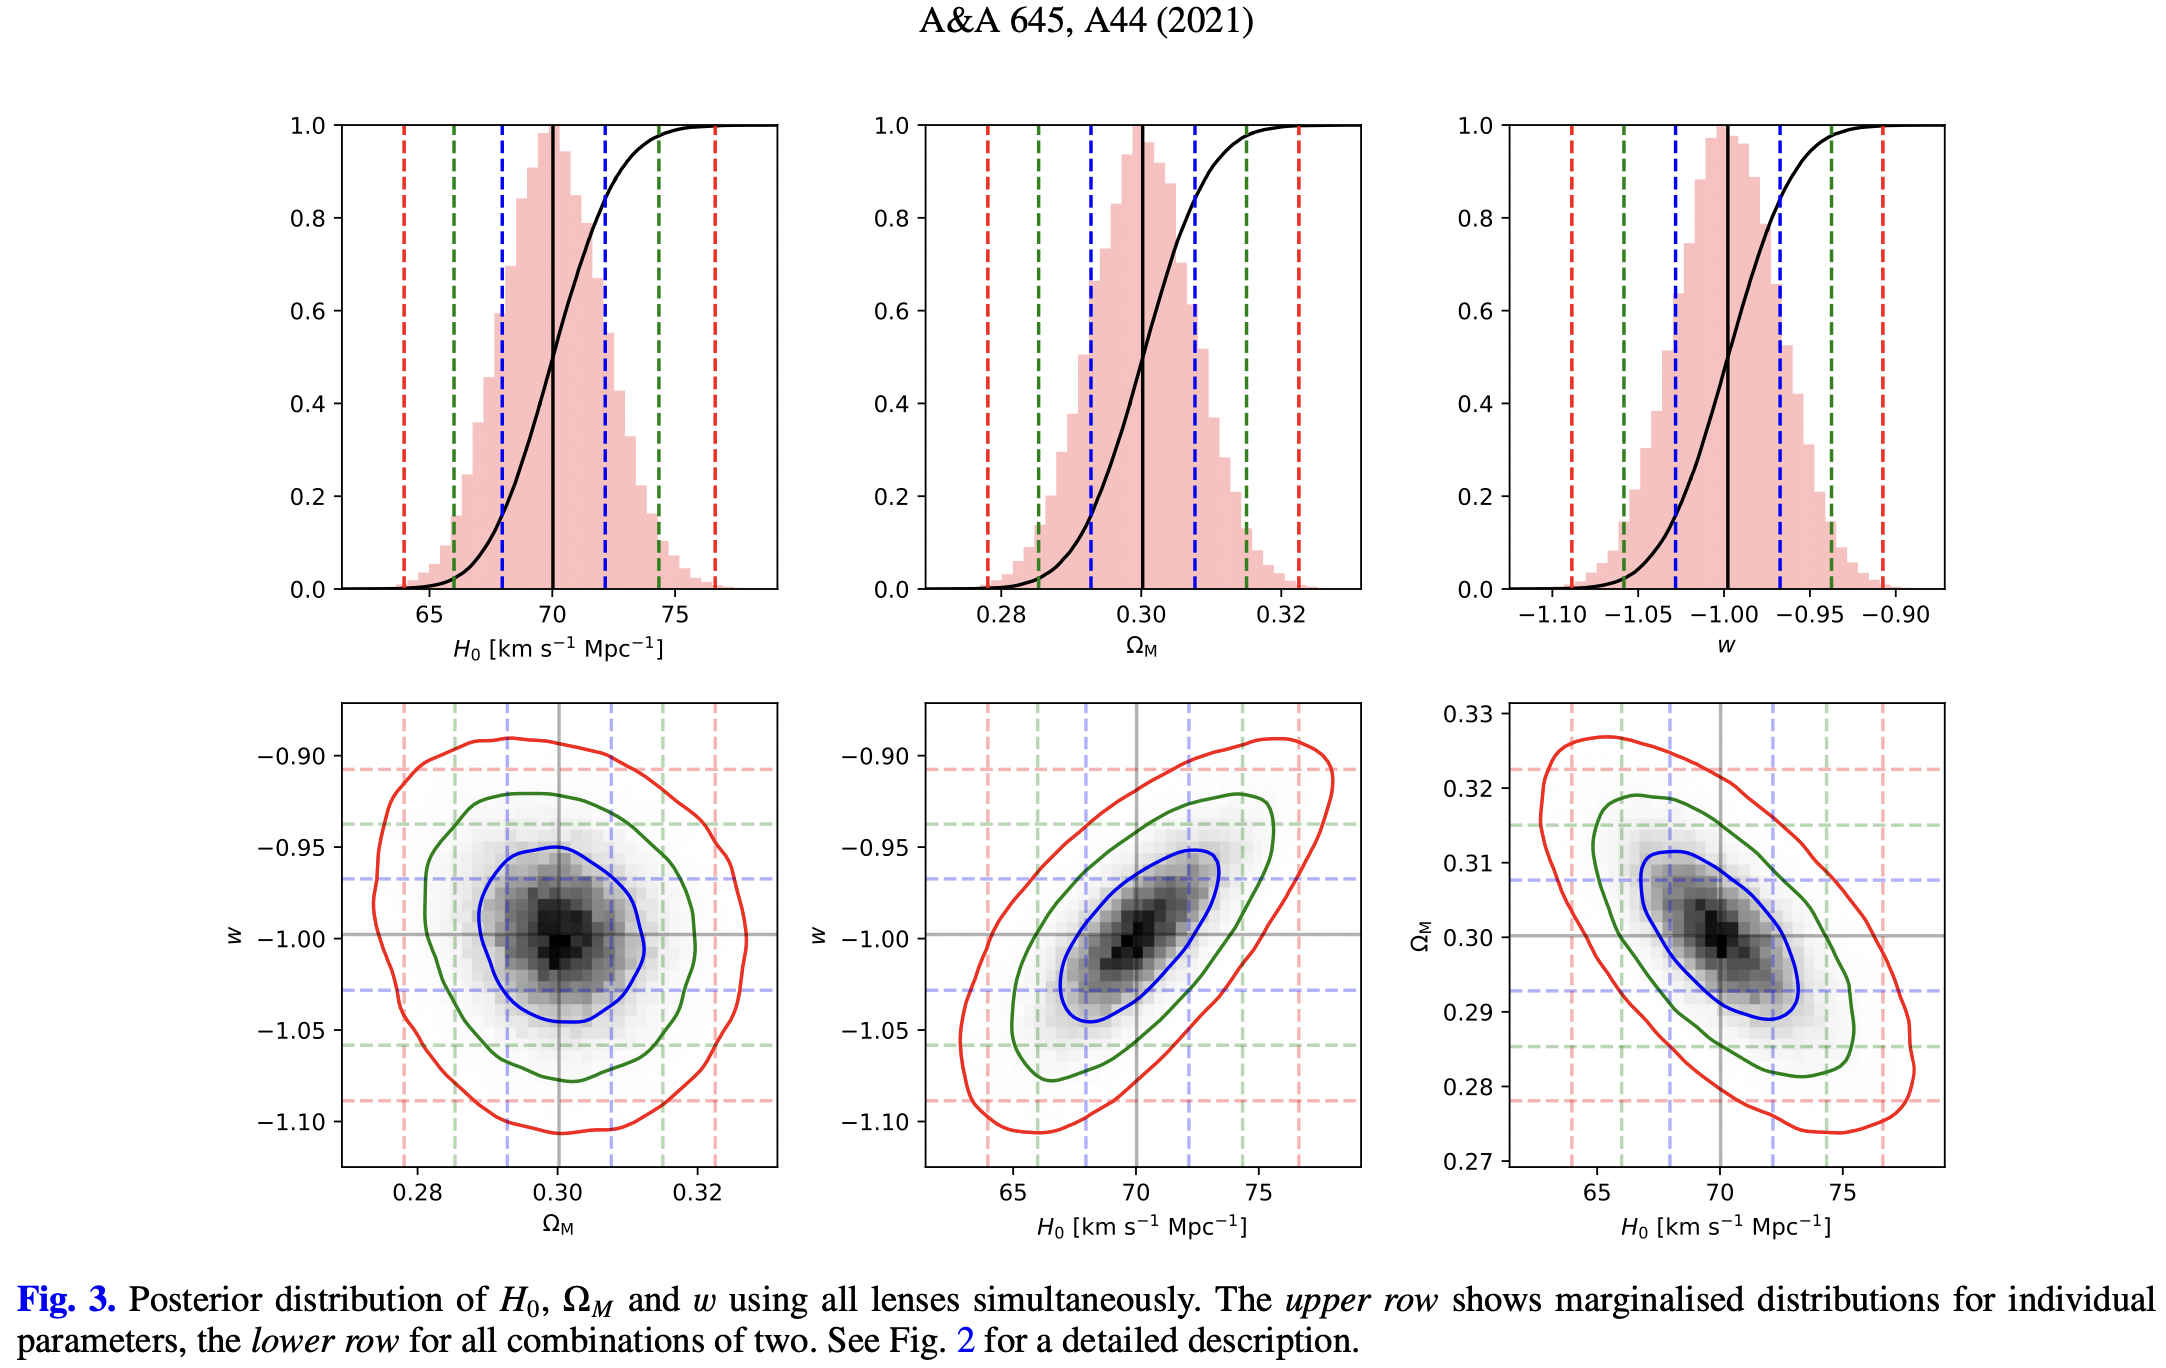
\includegraphics[width=4.5in]{Figures/wucknitz.png}

Wucknitz, Spitler, ULP 2021, A\&A, 645, A44
  }




  \frame{
    \frametitle{Catastrophes}
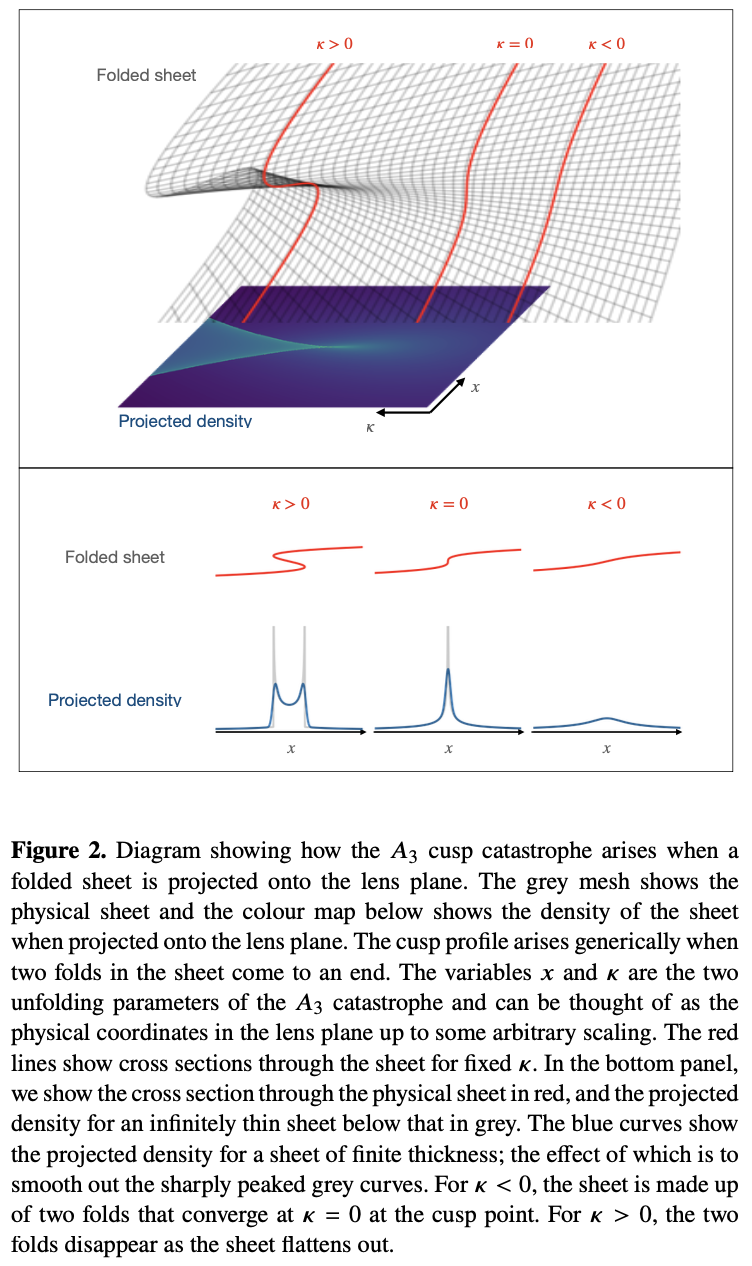
\includegraphics[width=2.85in]{Figures/cusp.png}
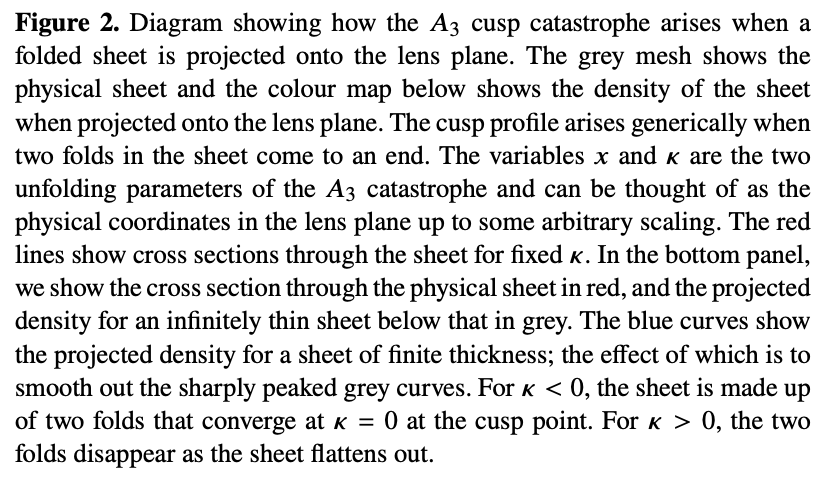
\includegraphics[width=0.5in]{Figures/cuspcaption.png}
Jow+22, in prep
  }




  \frame{
\vspace{-0.5in}
    \frametitle{Conclusions}
    \begin{itemize}
     \item wave optics changes nature of astrophysical observables: Coherent FRB/pulsar     radiation one of the potentially most
      precise measurements in physics
      \item already makes microarcsecond images of pulsars
      \item ISM plasma screens modelled quantitatively as localized
        1-D features, no longer stochastic turbulent volume.
      \item next generation FRB telescopes for cosmic mass inventory,
        possibly dark energy/acceleration
    \end{itemize}
  }

\end{document}
